\begin{introduction}
Rozpoznávání obrazu je bezesporu jedno z~aktuálně nejhojněji diskutovaných a~rychle se rozvíjejících témat posledních let. Prakticky denně lze sledovat nové metody a technologie tohoto oboru, které nám usnadňují práci a celkově mění náš život. Příkladem mohou být nově vznikající autonomní vozidla, která ke svému řízení využívají sadu senzorů a kamer, a mají za úkol nás co nejbezpečněji dopravit na potřebné místo. Jiným příkladem mohou být rozsáhlé neuronové sítě, které na základě vstupního obrázku zvládnou detekovat předměty, osoby a dokonce popsat činnosti, které se na snímku odehrávají. Zkrátka, oboru rozpoznávání obrazu se aktuálně věnuje velké množství lidí po celém světě a vzhledem k~tempu, jakým se všechny technologie vyvíjejí, je možné brzy očekávat převratné novinky s~užitkem pro lidstvo.

Další velmi zajímavou oblastí, která se v~posledních letech začíná značně rozšiřovat a přibližovat veřejnosti, jsou termokamery. Pomáhají nám při záchraně osob, v~průmyslu (například při monitorování nebezpečných látek), ale dokonce už i při běžných činnostech jako je hledání chyb v~tepelné izolaci našich domů.

Oblast termografie má za sebou již dlouhou řadu let výzkumu a vývoje. Zatímco infračervené záření bylo objeveno již kolem roku 1800, první prototypy kamer, které by infračervené záření zvládli zaznamenat, byly vynalezeny až kolem roku 1930. Od této doby technologie termokamer prošla několika generacemi, ale je zřejmé, že možnosti termokamer ještě nejsou zdaleka vyčerpány. Stále se objevují nové inovace a příkladem lze zmínit firmu FLIR Systems (dále jen FLIR), která je jedním z~největších výrobců termokamer na celém světě. FLIR postupně rozšiřuje své portfolio termokamer i~do neobvyklých oborů, jako jsou již zmíněná autonomní vozidla, ale snaží se zpřístupnit kamery i~pro širokou veřejnost. Jejich termografické moduly pro chytré telefony je možné pořídit za velmi lidovou cenu a jsou dostupné skoro pro každého. 

O~tom, že lidé o~obor termografie mají stále větší zájem svědčí i to, že firma FLIR v~roce 2014 představila svoji první verzi modulu pro chytré telefony a v~roce 2017  je už dostupná jeho třetí generace. V~roce 2016 byl dokonce představen i samostatný chytrý telefon s~již zabudovanou termokamerou. Je tedy zřejmé, že termokamery se velmi rychle rozšiřují do podvědomí veřejnosti a postupně se dále budou stávat již běžnou součástí dennodenních zařízení.

\begin{figure}
    \subfloat[FLIR One 3rd gen.]{{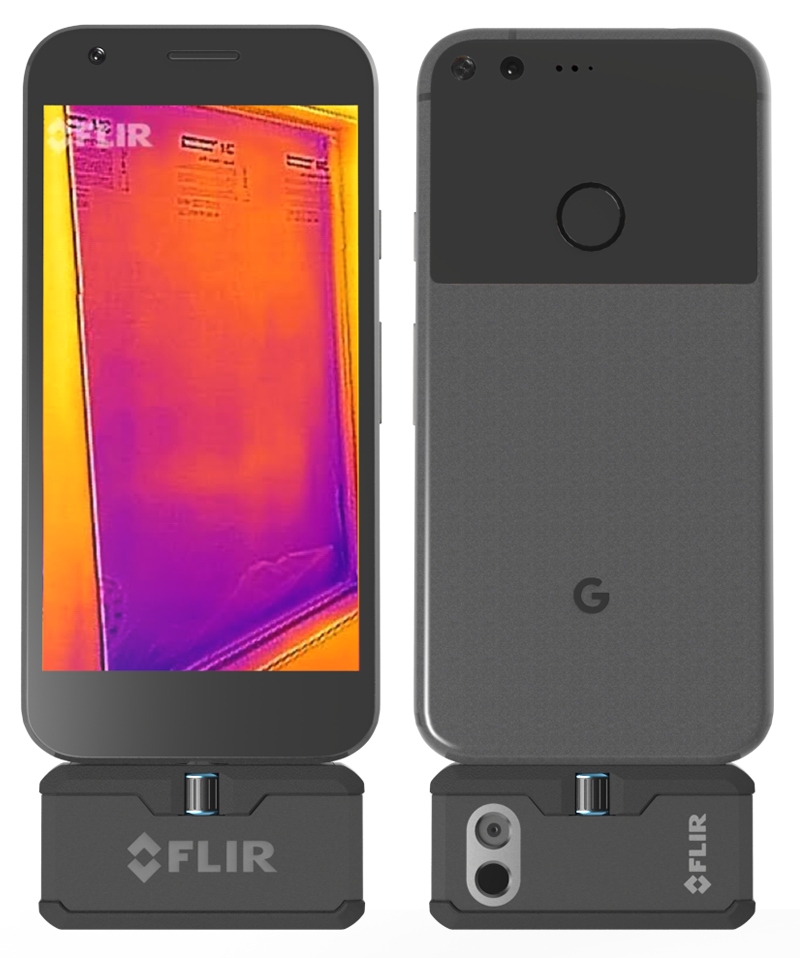
\includegraphics[width=5cm]{images/flir_one.png} }}
    \qquad
    \subfloat[CAT S60]{{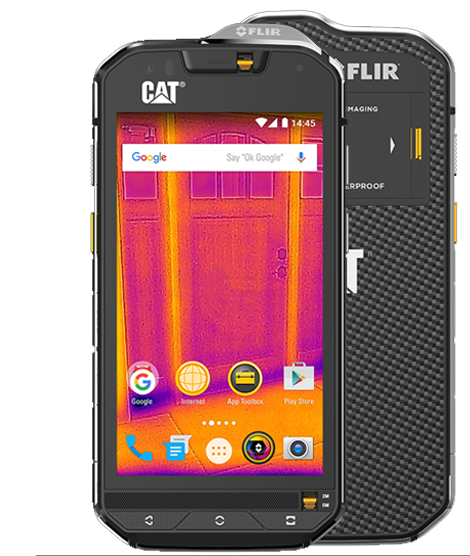
\includegraphics[width=5cm]{images/cat_s60.png} }}
    \caption{Na obrázku (a) je možné vidět přídavný modul pro chytré telefony a na (b) telefon s~již zabudovanou termokamerou}
    \label{fig:example}
\end{figure}

	\section{Motivace}
	Využití těchto nově rozvíjejících technologií by pro toto téma mělo přinést nové zajímavé objevy a poznatky k~ještě neúplně probádané oblasti. 
    
    Tématem detekce zboží v~ruce se již zabýval student Oliver Keruľ-Kmec ve své bakalářské práci \cite{kerul2016detekce}, ale bylo zjištěno, že se jedná o~poměrně náročnou úlohu. Jeho práce přináší řešení a poznatky, ale obecně je možné tvrdit, že problém ještě nebyl doposud uspokojivě vyřešen. Má tedy smysl se tématem dále zabývat a~to zejména na jiné úrovni obrazu než bylo řešeno, a tím je termografický obraz.
	
	\section{Cíl práce}
    Cílem práce je seznámení s~úlohou detekce zboží v~ruce zákazníka, prozkoumání souvisejících řešení úloh v~oblasti termokamer. Dále návrh vlastního algoritmu, který bude zboží v~ruce zákazníka schopný detekovat. Algoritmus bude implementován v~programovacím jazyku Java s~využitím volně dostupné knihovny OpenCV. Pro ověření funkčnosti algoritmu je nutné jeho vyhodnocení na vlastnoručně naměřených datech. Na základě dosažených výsledků bude provedena diskuze nad výhodami a nevýhodami využitého řešení.
    
	\section{Struktura dokumentu}
    V~první řadě je nutné obecné seznámení s~termokamerami a oblastí termografie. K~tomu slouží první kapitola, kde jsou stručně probrány důležité základy pro pochopení práce. Následně je provedena analýza zadaného problému, zavedení nutných předpokladů a představení prostředků práce. Nadcházející kapitola se pak věnuje průzkumu možných řešení a popisu navržených postupů. Ve čtvrté kapitole jsou  vyhodnoceny dosažené výsledky a pátá kapitola  je věnována  implementačním záležitostem. V~poslední části je celkové zhodnocení využitých postupů. 
    
	\section{Návaznost práce}
	Tato práce nepřímo navazuje na práci studenta Olivera Keruľ-Kmece \textit{Detekce přítomnosti zboží v~ruce zákazníka} \cite{kerul2016detekce}. 

\end{introduction}